\documentclass[aspectratio=169]{beamer}
\usepackage{goethecc}

\usepackage{color, colortbl}

\usepackage[USenglish]{babel}
\usepackage{amsmath,amsfonts,amssymb}
\usepackage{graphicx}
\usepackage{pdfpages}

\usepackage{latexsym}
\usepackage{xspace}

\usepackage{aurical}

%TODO: Cyriax should install packages...
%\usepackage{siunitx}
%\sisetup{locale = DE}

\usepackage{xstring}
\usepackage{tikz}
\usepackage{pgf}
\usetikzlibrary{calc}   
\usetikzlibrary{positioning}
\usetikzlibrary{automata}
\usetikzlibrary{arrows}   

\usepackage{soul}

\graphicspath{{./images/}}

\tikzset{onslide/.code args={<#1>#2}{%
    \only<#1>{\pgfkeysalso{#2}} % \pgfkeysalso doesn't change the path
}}
\tikzset{onslidep/.code args={<#1>#2}{%
		\ifthenelse{#1 = 0}{}{\only<#1->{\pgfkeysalso{#2}}} % \pgfkeysalso doesn't change the path
}}
\tikzset{onslidepp/.code args={<#1><#2>#3}{%
		\ifthenelse{#1=0 \OR #2=0}{}{\only<#1-#2>{\pgfkeysalso{#3}}} % \pgfkeysalso doesn't change the path
	}}
\tikzset{temporal/.code args={<#1>#2#3#4}{%
    \temporal<#1>{\pgfkeysalso{#2}}{\pgfkeysalso{#3}}{\pgfkeysalso{#4}} % \pgfkeysalso doesn't change the path
}}
\tikzset{onif/.code args={<#1>#2}{%
 	\ifthenelse{#1}{\pgfkeysalso{#2}}{}%
}}
 		
\def\cellSize{27pt}
\def\tmBlankSym{\ensuremath{\mathbb B}}
		
\tikzset{tmCell/.style={font={\Large\tt}, minimum height=\cellSize, minimum width=\cellSize}}
\tikzset{tmCellActive/.style={tmCell}}
\tikzset{tmCellBlank/.style={dunkelgrau!50, fill=sandgrau}}
\tikzset{tmHeadMarker/.style={circle, draw, ultra thick, emorot, minimum width=0.9*\cellSize, minimum height=0.9*\cellSize}}

 		
 		

\newcommand{\tikzanchor}[1]{\tikz[overlay, remember picture]{\node[anchor=text, inner sep=0] (#1) {\phantom{Ig}};}}

\newcommand{\tmstate}[4]{
	% 1 key
	% 2 label
	% tikz options
	% tikz position
	\node[
		tm-state,
		onif={<\equal{#1}{\tmStateCurrent}>tm-state-active},
		#3
	] (#1) #4 {#2};
}

\newcommand\tmstart[1]{
	\path[tm-trans]  ($(#1.west)-(1.5em, 0)$) to ++(1.5em, 0);
}

\newcommand{\trans}[3]{
	\def\transLabel{%
		\textbf{\texttt{#1}} zu \textbf{\texttt{#2}}, 
		\ifthenelse{\equal{#3}{L}}{$\Leftarrow$}{\ifthenelse{\equal{#3}{R}}{$\Rightarrow$}{$\Downarrow$}}%
	}%
	%
	\IfSubStr{\tmBand}{@#1@}
	{\ifthenelse{\tmTransOfCurrentState}{\textcolor{red}{\transLabel}}{\transLabel}}
	{\transLabel}
}

\newcommand{\tmtrans}[5]{
	% 1 current state
	% 2 next state
	% 3 instruction
	% 4 format path
	% 5 format label

   \def\tmTransOfCurrentState{\equal{\tmStateCurrent}{#1}}
   \def\tmConditionalTrans{}
   {
	   \renewcommand{\trans}[3]{%
		   \IfSubStr{\tmBand}{@##1@}{\ifthenelse{\tmTransOfCurrentState}{\global\def\tmConditionalTrans{tm-trans-active}{}}{}}{}%
	   }%
	   #3%
   }

   \path[tm-trans, \tmConditionalTrans] (#1) edge[#4] node[align=center, #5] {#3} (#2);
}

\newcommand{\turingBandActiveChar}[1]{
	\turingBandActiveCharHelp#1\relax\relax\relax\relax
}
\def\turingBandActiveCharHelp#1#2#3\relax{%
	\ifx#1\relax\else%
	\ifthenelse{\equal{#1}{@}}{#2}
	{\turingBandActiveCharHelp#2#3\relax\relax}%
	\fi%
}

\newcommand{\decreasedCounter}[1]{\numexpr\value{#1} - 1\relax}
\newcounter{tmbandcnt}
\newcounter{tmbandcntHead}

\newcommand{\tmbandCellCaption}[1]{%
	\ifthenelse{\equal{#1}{B}}{$\mathbb B$}{#1}%
}

\newcommand\turingBandNodes{
	\setcounter{tmbandcnt}{0}
	\setcounter{tmbandcnt}{0}
	\expandafter\turingBandHelp\tmBand\relax\relax\relax\relax
}
\def\turingBandHelp#1#2#3#4\relax{%
	\ifx#1\relax{}\else{%
		\stepcounter{tmbandcnt}
		\ifthenelse{\equal{#1}{@}}{%
			\node[tmcell-active, right=of tmbandcell-\the\decreasedCounter{tmbandcnt}] (tmbandcell-\thetmbandcnt) {\tmbandCellCaption#2};
			\setcounter{tmbandcntHead}{\thetmbandcnt}%
			\turingBandHelp#4\relax\relax\relax\relax%		
		}{%
		\node[tmcell, right=of tmbandcell-\the\decreasedCounter{tmbandcnt}] (tmbandcell-\thetmbandcnt) {\tmbandCellCaption#1};
		\turingBandHelp#2#3#4\relax\relax\relax%
	}%
}
\fi%
}

\newenvironment{tmStates}{
	\begin{tikzpicture}[
	node distance = 4em and 15em,
	on grid,
	tm-state/.style={draw, minimum width=6em},
	tm-state-active/.style={fill=red!50},
	tm-state-next/.style={blue},
	tm-trans/.style={draw, ->, ,shorten >=2pt, thick, auto},
	tm-trans-active/.style={red},
	loop above/.style={looseness=8, out=120, in=60},
	loop below/.style={looseness=8, out=300, in=240}
	]
}{
\end{tikzpicture}
}

\newcommand{\tmDrawBand}{
\begin{tikzpicture}[
	node distance=0,
	tmcell/.style={draw, minimum width=2em, minimum height=2em},
	tmcell-active/.style={tmcell},
	tmhead-marker/.style={draw, ultra thick, red, circle, minimum width=2.5em}
]
	\node (tmbandcell-0) {};
	\turingBandNodes
	\ifthenelse{\equal{\thetmbandcntHead}{0}}{}{
		\node[tmhead-marker, at=(tmbandcell-\thetmbandcntHead)] {};				
	}
\end{tikzpicture}
}


%%%%%%%%%%%% TM Execution

\def\tmMoveLeftHelp#1#2#3#4#5\relax{{%
	\ifx#1@%
		% Move left before start: Insert Blank Symbol
		\xdef\tmNewBand{@B@#2#4#5}%
	\else%
		\ifx#4\relax%
			% This is not possible in an input containing @
			ILLEGAL INPUT%
		\else
			\ifx#2@%
				\xdef\tmNewBand{\tmNewBand @#1@#3#5}%
			\else%
				\xdef\tmNewBand{\tmNewBand#1}%
				\tmMoveLeftHelp#2#3#4#5\relax\relax%
			\fi%
		\fi%
	\fi
}}

\def\tmMoveRightHelp#1@#2@#3#4\relax{{%
	\ifx#3\relax
		\xdef\tmNewBand{#1#2@B@}%
	\else
		\xdef\tmNewBand{#1#2@#3@#4}%
	\fi
}}

\newcommand{\tmMoveLeft}{%
	\def\tmNewBand{}%
	\expandafter\tmMoveLeftHelp\tmBand\relax\relax\relax\relax\relax%
	\xdef\tmBand{\tmNewBand}
}

\newcommand{\tmMoveRight}{%
	\def\tmNewBand{}%
	\expandafter\tmMoveRightHelp\tmBand\relax\relax\relax\relax\relax%
	\xdef\tmBand{\tmNewBand}
}


\def\tmCurrentCharHelp#1@#2@#3\relax{\xdef\tmHeadChar{#2}}%
\newcommand{\tmCurrentChar}{\expandafter\tmCurrentCharHelp\tmBand\relax}

\def\tmWriteCharHelp#1@#2@#3\relax{\xdef\tmBand{#1@\tmCharToWrite@#3}}%
\newcommand{\tmWriteChar}[1]{%
	\def\tmCharToWrite{#1}%
	\expandafter\tmWriteCharHelp\tmBand\relax%
}

\def\tmTrans#1#2#3#4#5\relax{
	\if\tmHeadChar#1
		\tmWriteChar#2
		\if#3L
			\tmMoveLeft
		\else\if#3R
			\tmMoveRight
		\fi\fi
		#4
	\else
		\if\relax\detokenize{#5}\relax\else
			\tmTrans#5\relax
		\fi
	\fi
}

\def\tmShowBandHelp#1@#2@#3\relax{%
	\texttt{#1\underline{#2}#3}%
}

\newcommand{\tmShowBand}{
	\expandafter\tmShowBandHelp\tmBand\relax	
}

\begin{document}
\title{
	Und womit rechnest du so? \\[-0.5em]
	\textcolor{dunkelgrau}{\small \emph{mit Folien von Cyriax und Manuel}}
}
\author{
	Jonathan Cyriax Brast\\
	Manuel Penschuck \\
} 
\date{10. Juni 2017}

{
\setbeamertemplate{footline}{} 
\goethccBgTitel
\begin{frame}
  \titlepage
  \begin{tikzpicture}[overlay]
	  \node[anchor=south east, xshift=-0.08\textwidth, yshift=0.05\textheight, at=(current page.south east)] {
\includegraphics[width=0.15\textwidth]{cs.pdf}};
  \end{tikzpicture}
\end{frame}
}
\addtocounter{framenumber}{-1}


%\frame{\frametitle{Outline}\tableofcontents}

%%%%%%%%%%%%%

\newcommand{\handwrittenNoteBelow}[3]{
	\node[goetheblau, anchor=west, align=left] at ($(#1)+(1.6,-0.6)#3$) {\Large \Fontauri\bfseries #2};
	\path[<-, draw, goetheblau, ultra thick, bend right=15] ($(#1)#3$) to ++(1.5,-0.5);
}

\newcommand{\handwrittenNoteAbove}[3]{
	\node[goetheblau, anchor=west, align=left] at ($(#1)+(1.6,0.6)#3$) {\Large \Fontauri\bfseries #2};
	\path[<-, draw, goetheblau, ultra thick, bend left=15] ($(#1)#3$) to ++(1.5,0.5);
}


\begin{frame}{}
	\begin{center}
		\Huge
		\only<1>{Turing Maschine}
		\only<2-3>{%
			\only<2>{\includegraphics[height=0.6\textheight]{images/cumberbatch.jpg}}%
			\only<3>{\includegraphics[height=0.6\textheight]{images/turing.jpg}}%
			\hspace{2em}
			\includegraphics[height=0.6\textheight]{images/nos2012.jpg}
			\vspace{1em}
						
			Alan M. Turing\\
			1912 -- 1954 
		}
		\only<4>{
			\fbox{\includegraphics[height=0.6\textheight]{images/turing1936.png}}
			\vspace{1em}
			
			\textquotedblleft On Computable Numbers, With an Application to the Entscheidungsproblem\textquotedblright\\
			\textcolor{goetheblau}{[A. Turing, 1936/37]}
		}
	\end{center}
\end{frame}


\begin{frame}{Turing Maschine}
	\begin{center}
		\vspace{2em}

		\uncover<7->{
			\begin{tikzpicture}[remember picture]
				\node[tmState, draw] (stateA) {Zustand A};
				\node[tmState, draw, anchor=west] (stateB) at ($(stateA.east) + (5,0)$)  {Zustand B};
				
				\path[draw, ->, thick, bend left=10, shorten >=5pt, onslide={<8>, emorot}] (stateA) to node[above] {\tikzanchor{transAnchor} \texttt 0 zu \texttt 1, $\Rightarrow$} (stateB);
				\path[draw, ->, thick, bend left=10, shorten >=5pt] (stateB) to node[below,align=left] {\texttt 0 zu \texttt 0, $\Leftarrow$ \\ \texttt 1 zu \texttt 1, $\Leftarrow$} (stateA);
			\end{tikzpicture}

			\begin{tikzpicture}[remember picture, overlay]
				\handwrittenNoteBelow{stateB}{Programm}{-(2,1)}
							
			
				\only<8->{
					\handwrittenNoteAbove{transAnchor}
					{\normalfont\normalsize Wenn \textcolor{emorot}{\texttt 0} gelesen:\\ Schreibe \textcolor{emorot}{\texttt 1}, Kopf nach rechts}
					{+(1.8,0.2)}
				}
			\end{tikzpicture}			
		}

		\vspace{3em}
		
		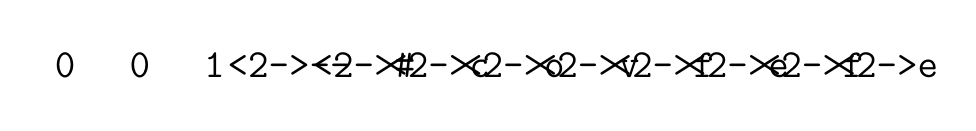
\begin{tikzpicture}[
			remember picture
		]
			\node[tmCell                ] (tmbandcell0) {};		

			\foreach \x  [count=\i] in {
				0,0,1,
				\only<2->{--},
				\only<2->{\#},
				\only<2->{c},
				\only<2->{o},
				\only<2->{v},
				\only<2->{f},
				\only<2->{e},
				\only<2->{f},
				\only<2->{e}
			} {
				\node[tmCell] at ($(tmbandcell0) + (\i*\cellSize,0) - (\cellSize,0)$) {\x};
			}
		\end{tikzpicture}
			

		\begin{tikzpicture}[overlay, remember picture]
			\only<1-2> {
				\handwrittenNoteBelow{tmbandcell0}{Eingabe}{+(2, -0.6)}
			}
		
			\only<1> {\tmDrawGrid{0}{3}}
			\only<2> {\tmDrawGrid{0}{12}}
			\only<3-> {
				\foreach \i in {1,...,5} {
					\node[tmCell, tmCellBlank] at ($(tmbandcell0) - (\i*\cellSize,0)$) {\only<4->{\tmBlankSym}};
					\node[tmCell, tmCellBlank] at ($(tmbandcell0) + (\i*\cellSize,0) + (11*\cellSize, 0)$) {\only<4->{\tmBlankSym}};
				}
				\tmDrawGrid{-5}{18}

				\handwrittenNoteBelow{tmbandcell0}{Speicher / Band}{+(2, -0.6)}
			}
			
			\only<5->{
				\node[tmHeadMarker, at=(tmbandcell0)] {};
				\handwrittenNoteAbove{tmbandcell0}{Kopf}{+(0.4, 0.4)}
			}
			
			\only<6->{
				\node[emorot, anchor=north, at=(tmbandcell0.south), yshift=-0.2em] {\Large $\Leftarrow, \Downarrow, \Rightarrow$};
			
			}
		\end{tikzpicture}
	\end{center}
\end{frame}
\def\turingAStateDef{
%%%%%% BEGIN-TM: turingI, B111-11B %%%%%
	\tmstate{firstMinus}{Suche Minus}  {}{}
	\tmstate{rightDigit}{Rechte Ziffer}{above right=of firstMinus}{}
	\tmstate{leftDigit} {Linke Ziffer} {below right=of firstMinus}{}
	\tmstate{cleanUp}   {Aufräumen}    {below right=of rightDigit}{}
	
	\tmstart{firstMinus}
	
	\tmtrans{firstMinus}{firstMinus}{\trans 11R }{loop below}{}
	\tmtrans{firstMinus.east}{rightDigit.west}{\trans --R}{above,sloped}{}
	
	\tmtrans{rightDigit}{rightDigit}{\trans --R}{loop above}{}
	\tmtrans{rightDigit}{leftDigit}{\trans 1-L}{bend right, below, left}{}
	\tmtrans{rightDigit.east}{cleanUp.west}{\trans BBL}{above, sloped}{}
	
	
	\tmtrans{leftDigit}{leftDigit}{\trans --L}{loop below}{}
	\tmtrans{leftDigit}{rightDigit}{\trans 1-R}{bend right, below, right}{}
	
	\tmtrans{cleanUp}{cleanUp}{\trans -BL}{loop below}{}
%%%%%% END-TM: turingI %%%%%
}

\newcommand{\tmADraw}[1]{
	\newcommand{\tmStateCurrent}{#1}

	\begin{center}
		\scalebox{0.8}{
			\tmDrawStates{\turingAStateDef}
		}			
		
		\scalebox{0.8}{
			\tmDrawBand
		}
	\end{center}
}


\newcommand{\tmACallback}[1]{\only<+>{\tmADraw{#1}}}
\tmSetup{A}{\turingAStateDef}

\begin{frame}{Unäre Subtraktion}
	\tmExecute{A}{111-11B}{\tmACallback}
\end{frame}

\begin{frame}{Hier könnte Ihre Werbung stehen}
$1+1=10$
\end{frame}
\newcommand{\bsl}{\textbackslash}

\begin{frame}{sed - h\"a, was?}
	sed steht f\"ur Stream Editor\\
	also:\\
	sed nimmt sich einen Textstrom und pfuscht in dem irgendwie rum:\\
	Beispiel:\\
	\texttt{s/2016/2017/} = Suche 2016 und ersetze es mit 2017\\
	''NoS Vortrag 2016'' $\rightarrow$ ''NoS Vortrag 2017''\\
\end{frame}


%TODO: braucht noch: wenn ich nichts finde passiert nichts...
\begin{frame}{Editwar mit sed}
	''Manu ist der Beste!''\\
	\quad\quad\texttt{s/der Beste/doof/}\\
	''Manu ist doof!''\\
	\quad\quad\texttt{s/Manu/Cyriax/}\\
	''Cyriax ist doof!''\\
	\quad\quad\texttt{s/ist doof/hat Manus Vortrag gekapert/}\\
	''Cyriax hat Manus Vortrag gekapert!''\\
	\quad\quad\texttt{s/(.*) hat (.*)s Vortrag gekapert/\bsl2 hat \bsl1s Vortrag gekapert/}\\
	''Manu hat Cyriaxs Vortrag gekapert!''
	\quad\quad\texttt{s/(.*) hat (.*)s Vortrag gekapert/\bsl2 hat \bsl1s Vortrag gekapert/}\\
	''Cyriax hat Manus Vortrag gekapert!''
\end{frame}

\begin{frame}{Turingmaschine Idee}
	Wir brauchen also:\\
	1. Zustand\\
	2. Zustands\"uberg\"ange\\
	2. Band\\
	3. Kopf\\
\end{frame}

\begin{frame}{Turingmaschine Zust\"ande}
	%TODO tikz Bild NeuerZustand0 <-0A- AlterZustand -1B-> NeuerZustand1
	Wir merken uns den Zustand und den Rest vom Wort:\\
	''ZUSTAND:X''\\
	Jeder \"Ubergang ist ein Suchen und Ersetzen:\\
	\texttt{s/AlterZustand:0/NeuerZustand0:A/}\\
	\texttt{s/AlterZustand:1/NeuerZustand1:B/}
\end{frame}

\begin{frame}{Turingmaschine BandKopfApparat}
	%\begin{dummeIdee}
	@ sieht aus wie ein Kopf...\\
	%\end{dummeIdee}
	Nach links gehen:\\
	''Hallo W@elt'' $\rightarrow$ ''Hallo @Welt''\\
	\texttt{s/(.*)(.)@(.*)/\bsl1@\bsl2\bsl3/}\\
	e lesen und \"a schreiben:\\
	''Hallo W@elt'' $\rightarrow$ ''Hallo W@\"alt''\\
	\texttt{s/(.*)@e(.*)/\bsl1@\"a\bsl2/}\\
	Beides Zusammen:
	''Hallo W@elt'' $\rightarrow$ ''Hallo @W\"alt''\\
	\texttt{s/(.*)(.)@e(.*)/\bsl1@\bsl2\"a\bsl3/}\\


\end{frame}






\end{document}

